% !TEX options=--shell-escape
	\documentclass{article}
	\usepackage{amsmath,amssymb}
	\usepackage[inline]{enumitem}
	\usepackage{blindtext}
	\usepackage{booktabs}
	\usepackage{graphicx}
	\usepackage{xcolor}
	\usepackage[vmargin = 1.5in, top = 1in, bottom = 1.2in, letterpaper]{geometry}
	\usepackage{listings}
	\usepackage{courier}
	\usepackage{multicol}
	\usepackage{multirow}
	\usepackage{bm}
	\usepackage[labelformat=simple]{subcaption}
	\renewcommand\thesubfigure{(\alph{subfigure})}
	\usepackage{minted}
	\usepackage{fvextra}
	\definecolor{bg}{rgb}{0.95,0.95,0.95}
	\newminted{r}{mathescape, breaklines, linenos = true, bgcolor = bg}
	\usemintedstyle{tango}
	% \lstset{
	% basicstyle = \small\tt,
	% keywordstyle = \tt\color{blue},
	% commentstyle = \it\color[cmyk]{1,0,1,0},
	% stringstyle = \tt\color[RGB]{128,0,0},
	% %frame = single,
	% backgroundcolor = \color[RGB]{245,245,244},
	% breaklines,
	% extendedchars = false,
	% xleftmargin = 2em,
	% xrightmargin = 2em,
	% aboveskip = 1em,
	% tabsize = 4,
	% showspaces = false
	% }
	\newcommand\inner[2]{\left\langle{#1},{#2}\right\rangle}
	\DeclareMathOperator{\Corr}{Corr}
	\DeclareMathOperator{\Cov}{Cov}
	\DeclareMathOperator{\Var}{Var}
	\DeclareMathOperator{\E}{E}



	\begin{document}
	
	% \newfontfamily\courier{Courier New}

	
	\title{STAT 501 Exam 1}
	\author{Yifan Zhu}
	\maketitle
	
	\begin{enumerate}[leftmargin = 0 em, label = \arabic*., font = \bfseries]
	\item We plot the radial visualization and star coordinate plot to have an overview about the data set.
	\begin{rcode}
# read the data
skulls <- read.table("./Egyptian-skulls.dat")
names(skulls) <- c("max breadth", "basibregmatic height", "basialveolar length", "nasal height", "period")
skulls$period <- as.factor(skulls$period)

# visualization
## radial visualization
library(dprep)
source("radviz2d.R")
radviz2d(skulls, name = "Skulls")
## star plot
source("starcoord.R")
starcoord(data = skulls, class = TRUE, main = "Star coordinate plot for Skulls")
	\end{rcode}
	The data visualizations are shown in Figure~\ref{radviz_stars}.
	\begin{figure}[!htb]
	    \centering
		\begin{subfigure}[b]{0.5\textwidth}
		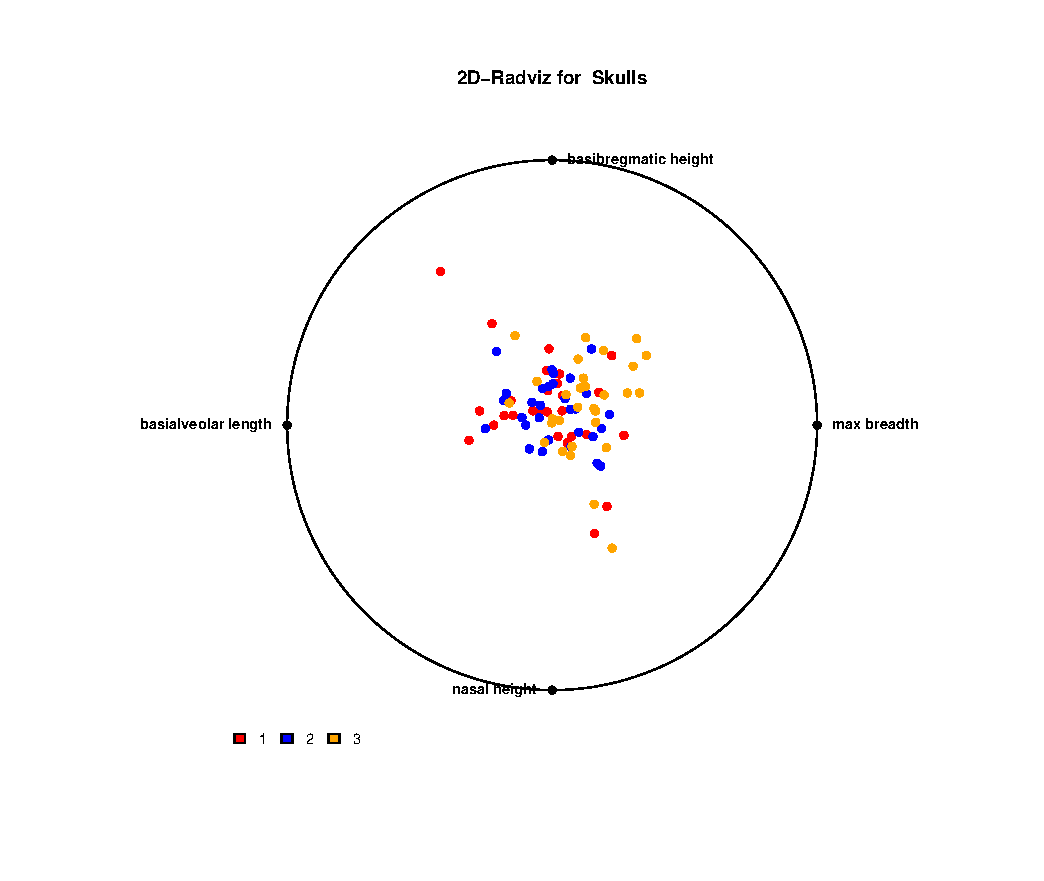
\includegraphics[width = \textwidth]{radviz.eps}
		\caption{radial visualization of skulls}
		\end{subfigure}%
		\begin{subfigure}[b]{0.5\textwidth}
		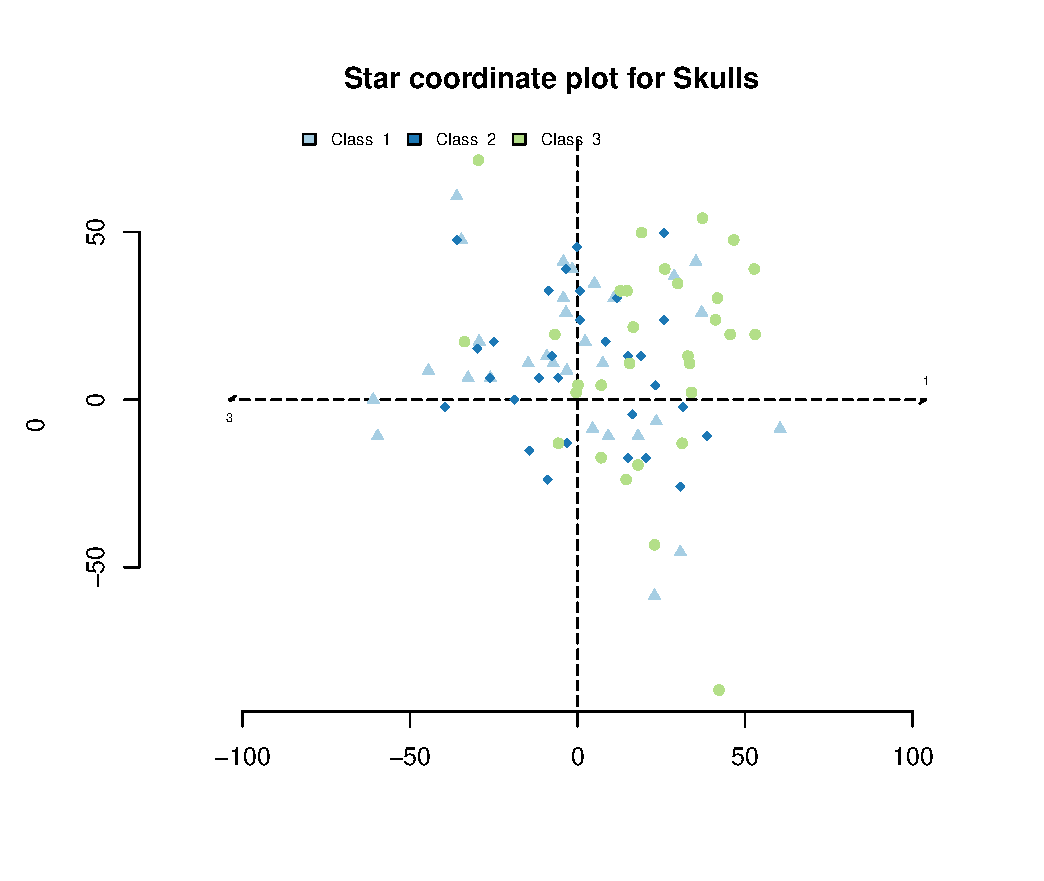
\includegraphics[width = \textwidth]{starcoord.eps}
		\caption{star coordinate plot of stars}
		\end{subfigure}
		\caption{data visualizations of skulls}
		\label{radviz_stars}
	\end{figure}

	From these two plots, we can not really see the difference among the three periods. They are mixed together and cannot be distinguished. We can also see from the two plots there is no big difference in the variability in these three periods (spread of data points are similar). 

	In order to check the distributional assumption of multivariate normality, we also plot the scatter plots in pairs and the $\chi^2$ Q-Q plots. See Figure~\ref{scatter} and Figure~\ref{QQ}.

	\begin{rcode}
## paired scatter plots
pairs(~., data = skulls[skulls$period == 1, -ncol(skulls)])
pairs(~., data = skulls[skulls$period == 2, -ncol(skulls)])
pairs(~., data = skulls[skulls$period == 3, -ncol(skulls)])
## Chi-squared Q-Q plot
library(MVN)
mvn(data = skulls[skulls$period == 1, -ncol(skulls)], multivariatePlot = "qq")
mvn(data = skulls[skulls$period == 2, -ncol(skulls)], multivariatePlot = "qq")
mvn(data = skulls[skulls$period == 3, -ncol(skulls)], multivariatePlot = "qq")
	\end{rcode}
	\begin{figure}[!htb]
	    \centering
		\begin{subfigure}[b]{0.33\textwidth}
		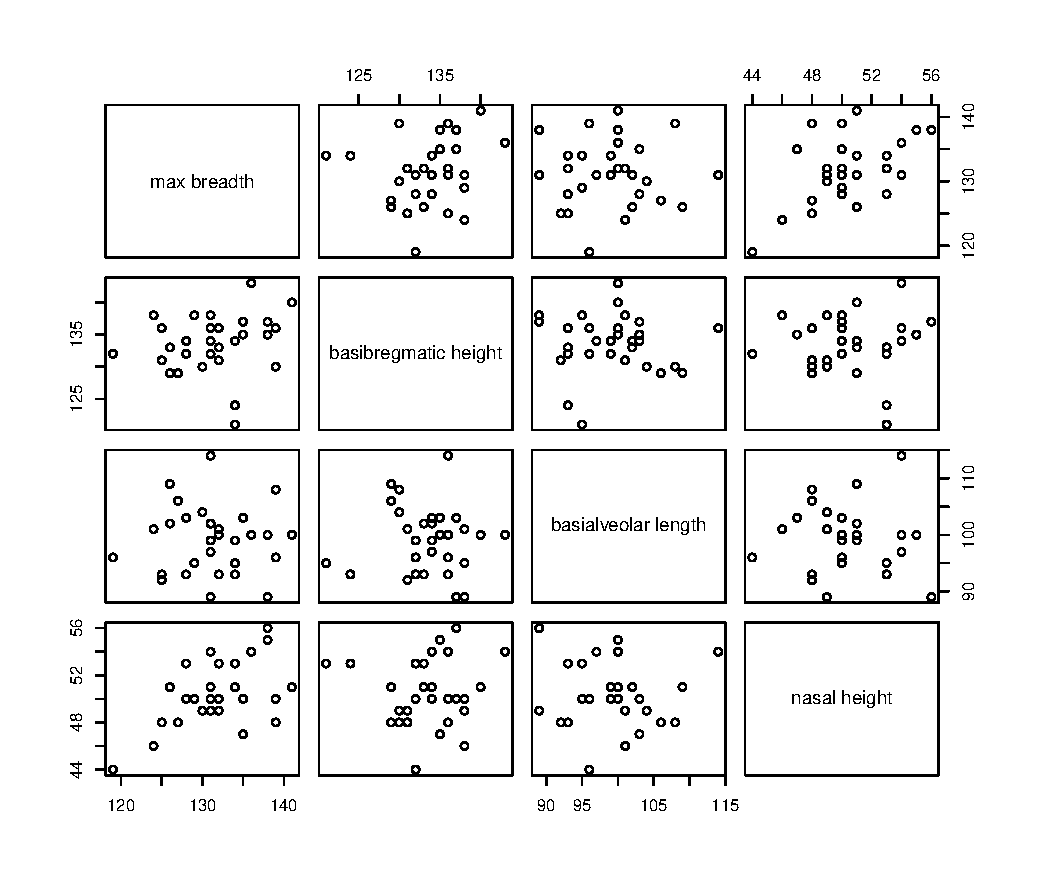
\includegraphics[width = \textwidth]{scatter_1.eps}
		\caption{period 1}
		\end{subfigure}%
		\begin{subfigure}[b]{0.33\textwidth}
		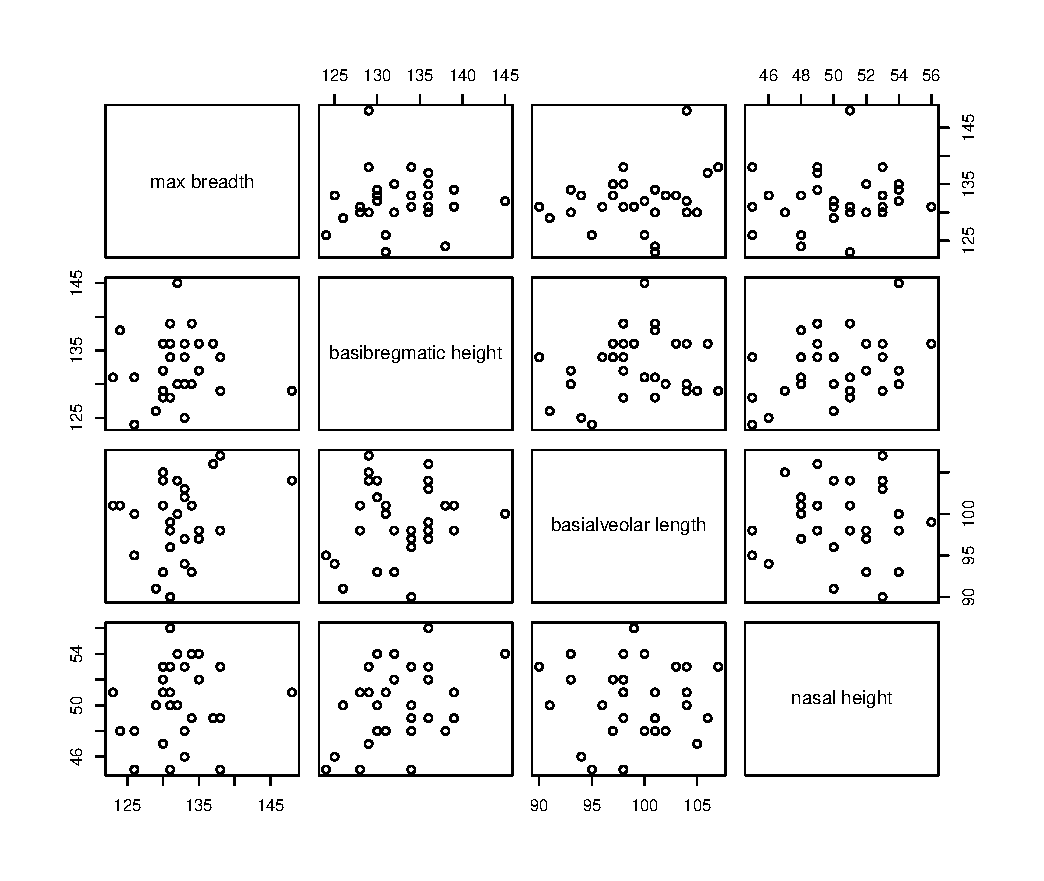
\includegraphics[width = \textwidth]{scatter_2.eps}
		\caption{period 2}
		\end{subfigure}%
		\begin{subfigure}[b]{0.33\textwidth}
		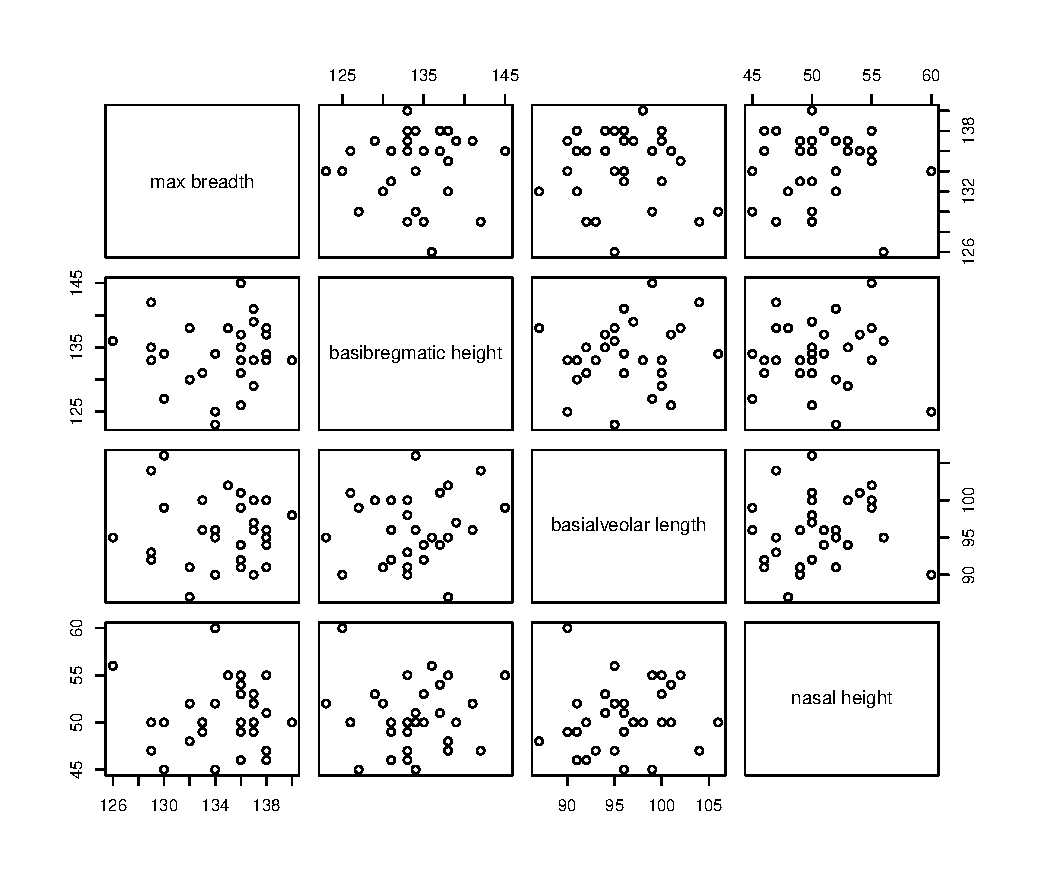
\includegraphics[width = \textwidth]{scatter_3.eps}
		\caption{period 3}
		\end{subfigure}
		\caption{paired scatter plots for 3 periods}
		\label{scatter}
	\end{figure}
	\begin{figure}[!htb]
	    \centering
		\begin{subfigure}[b]{0.33\textwidth}
		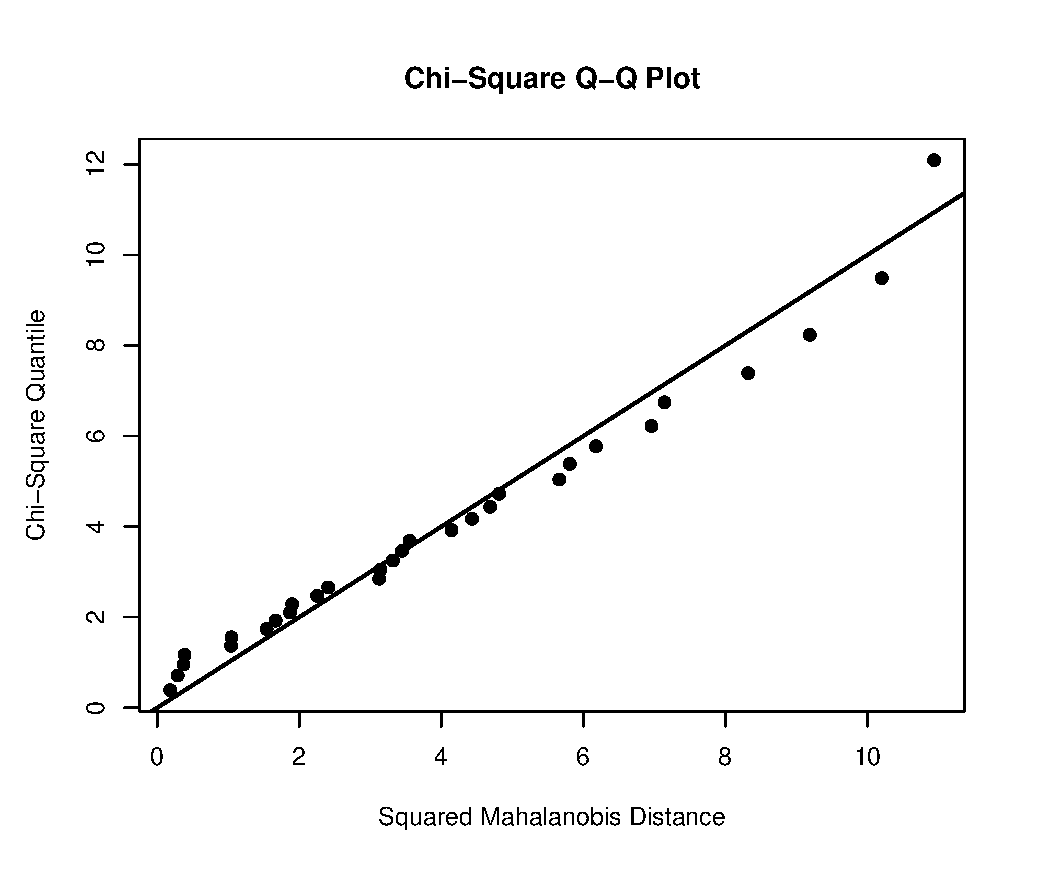
\includegraphics[width = \textwidth]{QQ_1.eps}
		\caption{period 1}
		\end{subfigure}%
		\begin{subfigure}[b]{0.33\textwidth}
		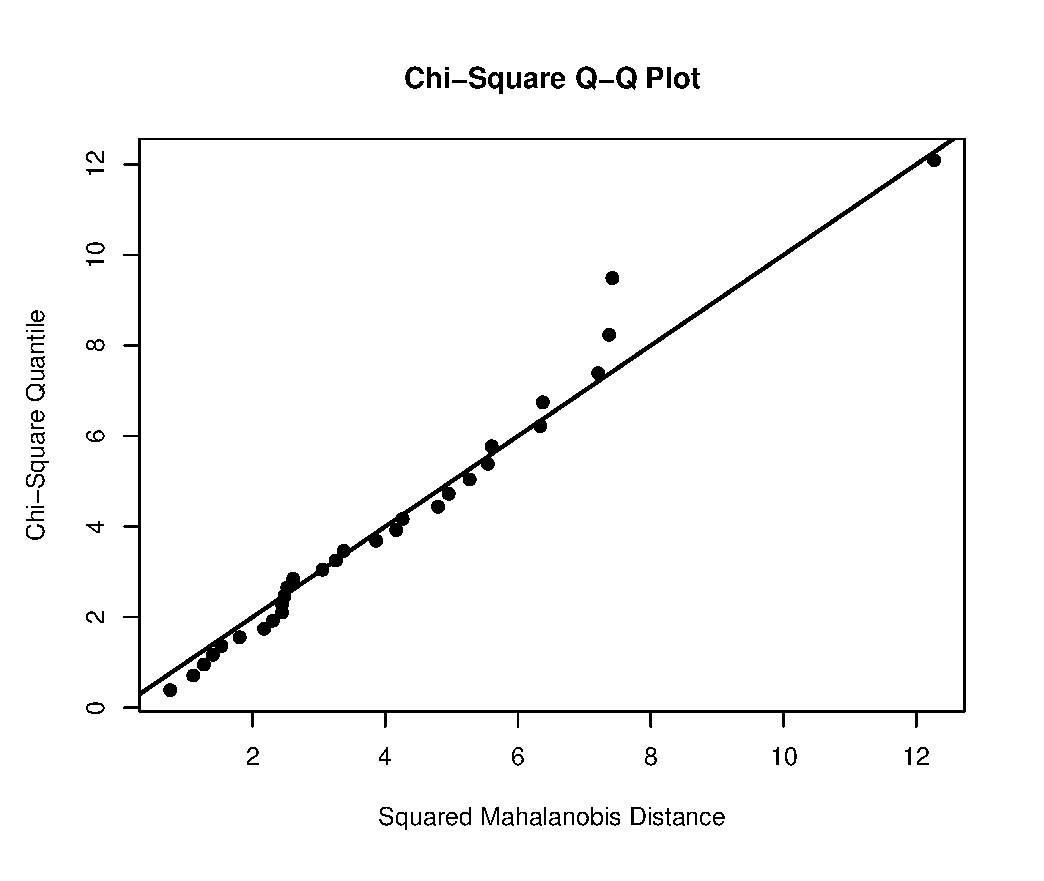
\includegraphics[width = \textwidth]{QQ_2.eps}
		\caption{period 2}
		\end{subfigure}%
		\begin{subfigure}[b]{0.33\textwidth}
		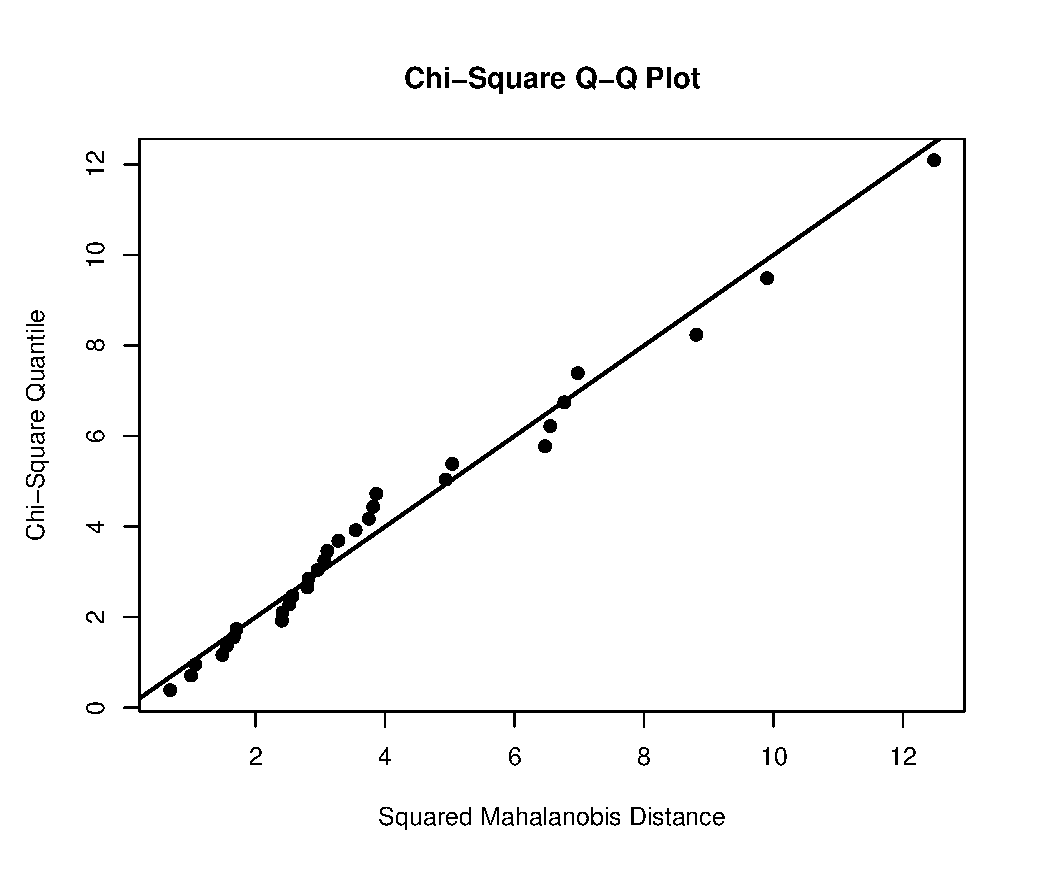
\includegraphics[width = \textwidth]{QQ_3.eps}
		\caption{period 3}
		\end{subfigure}
		\caption{$\chi^2$ Q-Q plots for 3 periods}
		\label{QQ}
	\end{figure}

	From Figure~\ref{scatter} we can see there is no strong linear relationship between any pairs in each time period, but we cannot really see the ellipse shape in the scatter plots, so we are not sure if the distribution is likely to be a multinormal from here. However, in Figure~\ref{QQ}, we can see the points fall around the straight line pretty well. So the multivariate normality might be reasonable here. 

\newpage
	\item 
	\begin{enumerate}
		\item 
		We conduct a formal test for each of the 3 time periods to test the multivariate normality.
		\begin{rcode}
## test for multivariate normality
source("testnormality.R")
testnormality(X = skulls[skulls$period == 1, -ncol(skulls)])
testnormality(X = skulls[skulls$period == 2, -ncol(skulls)])
testnormality(X = skulls[skulls$period == 3, -ncol(skulls)])
		\end{rcode}
		And the results (p-values) for 3 periods are \textbf{0.8585479} (period 1), \textbf{0.7971105} (period 2) and \textbf{0.506012} (period 3). With big p-values, we do not have significant evidence to reject the null hypothesis and conclude that the multivariate normality is reasonable for all 3 time periods. Same conclusion can be made from the $\chi^2$ Q-Q plots in Figure~\ref{QQ}.

		\item 
		We use Box M test to test the homogeneouity of dispersions. 
		\begin{rcode}
## test for homogeneouity of dispersions among 3 periods
source("BoxMTest-2.R")
BoxMTest(X = skulls[, -ncol(skulls)], cl = skulls$period)
		\end{rcode}
		The result is
		\begin{rcode}
[1] 3
------------------------------------------------
 MBox Chi-sqr. df P
------------------------------------------------
   22.5334    21.0484          20       0.3943
------------------------------------------------
Covariance matrices are not significantly different.
$MBox
      1 
22.5334 

$ChiSq
       1 
21.04844 

$df
[1] 20

$pValue
        1 
0.3942866 
		\end{rcode}
		So with big p-value, there is no significant evidence that the dispersions of the 3 time periods are different. We then plot the correlation plots for 3 time periods to see if there are any difference or redundancies. Plots are shown in Figure~\ref{corrplot}.
		\begin{rcode}
## correlation plot
source("plotcorr.R")
plot.corr(xx = skulls[skulls$period == 1, - ncol(skulls)])
plot.corr(xx = skulls[skulls$period == 2, - ncol(skulls)])
plot.corr(xx = skulls[skulls$period == 3, - ncol(skulls)])
		\end{rcode}
		\begin{figure}[!htb]
		    \centering
			\begin{subfigure}[b]{0.33\textwidth}
			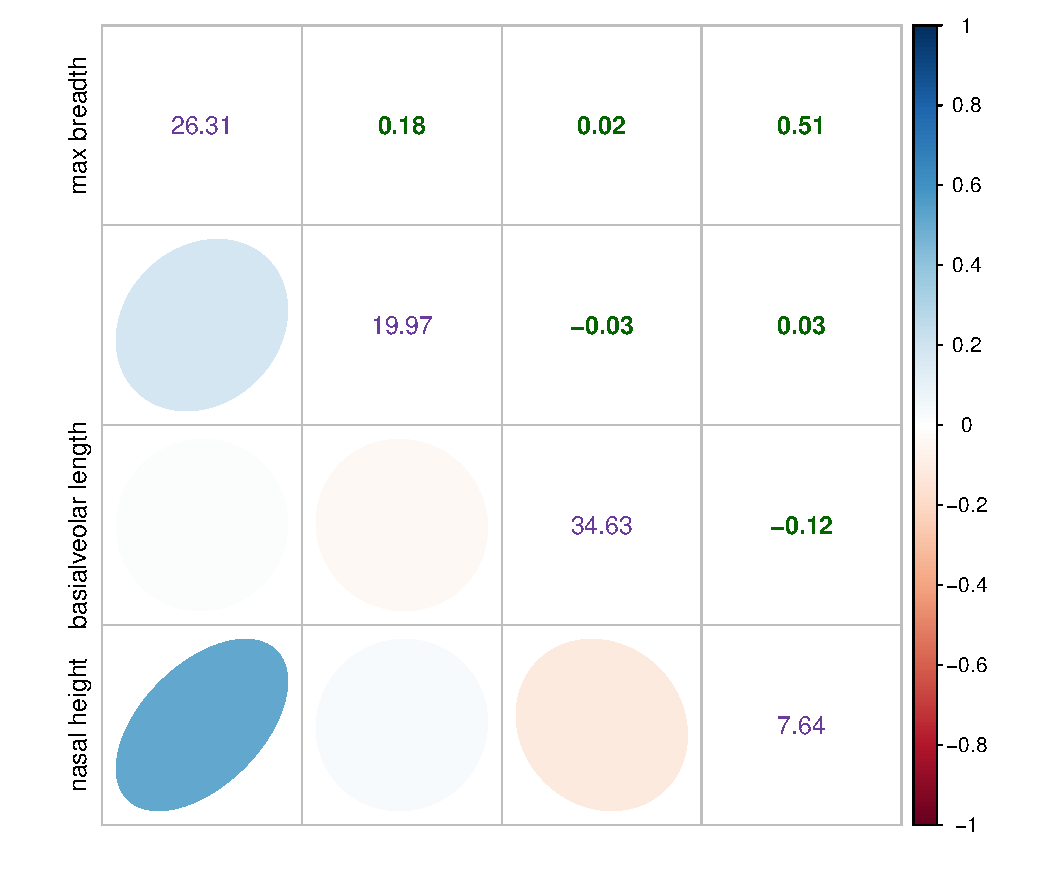
\includegraphics[width = \textwidth]{coorplot_1.eps}
			\caption{period 1}
			\end{subfigure}%
			\begin{subfigure}[b]{0.33\textwidth}
			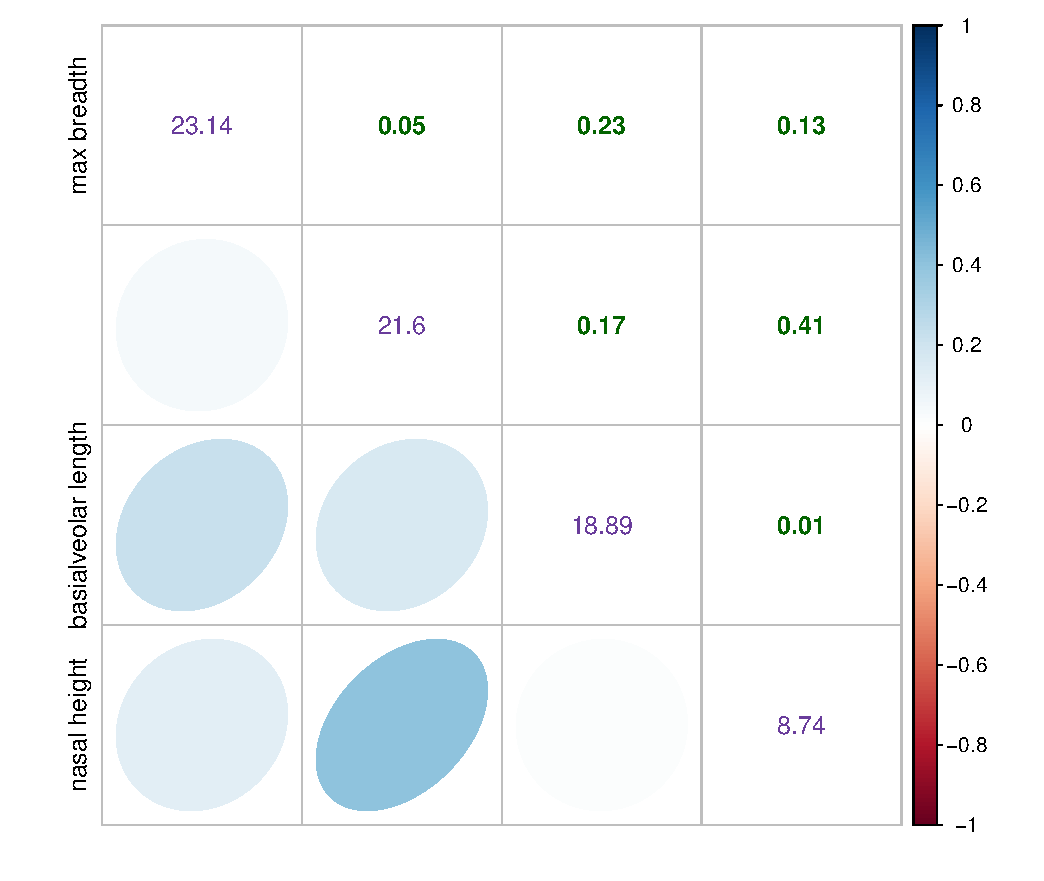
\includegraphics[width = \textwidth]{coorplot_2.eps}
			\caption{period 2}
			\end{subfigure}%
			\begin{subfigure}[b]{0.33\textwidth}
			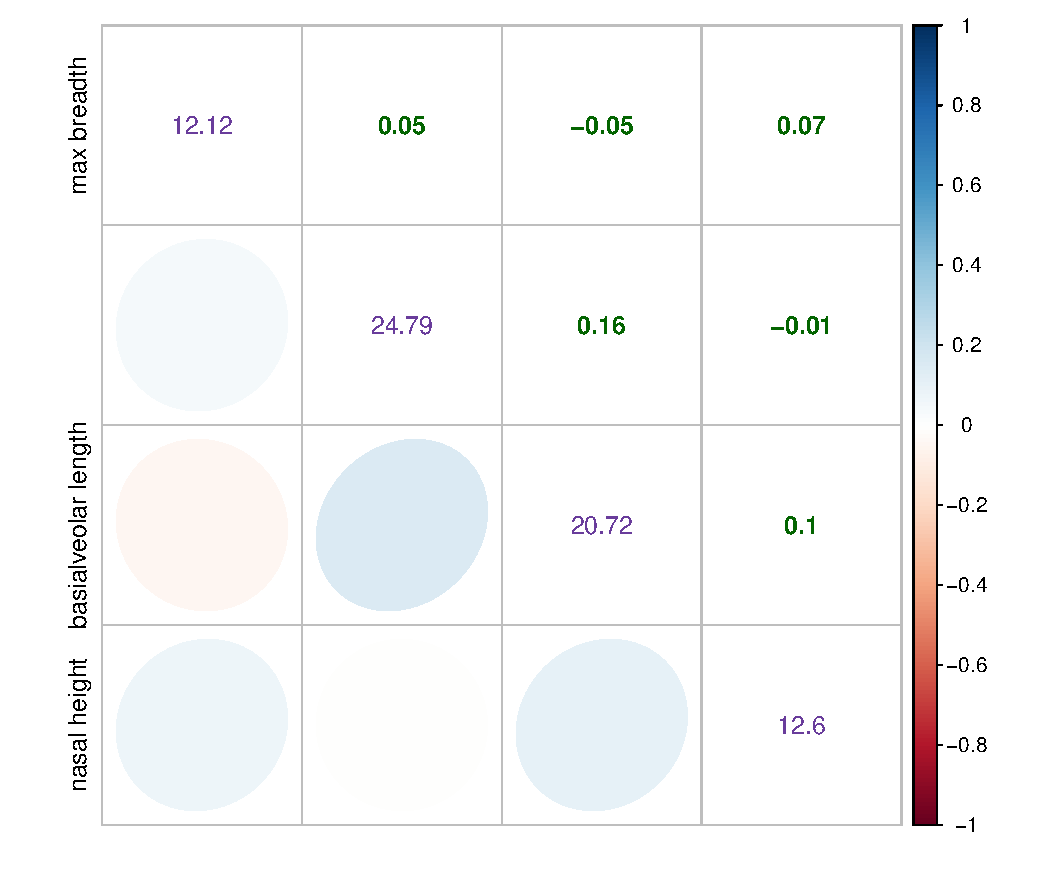
\includegraphics[width = \textwidth]{coorplot_3.eps}
			\caption{period 3}
			\end{subfigure}
			\caption{correlation plots for 3 time periods}
			\label{corrplot}
		\end{figure}

		From the correlation plots in Figure~\ref{corrplot}, we can see some difference in the correlations and variances for the 3 time periods. For example, the correlation between nasal height and maximun breadth for period 1 is higher than that of period 2 and period 3; the variance of maximum breadth for period 3 is smaller than that for period 1 and period 2; the correlation between nasal height and  basibregmatic height for period 2 is higher then that of period 1 and period 3 and so on. 

		And from the correlation plots we can also see that there is no redundencies. Although there are some correlations with absolute value around 0.5 (nasal height and maximum breadth for period 1), but the correlation of the same pair of measurements do not have big absolute value for all 3 periods, so there should be no linear relationship between these two measurements. This can also be seen from the scatter plots in Figure~\ref{scatter}.

	\end{enumerate}

	\item 
	We display the means of measurements in 3 time periods with star plots and Cheroff faces in Figure~\ref{display_means}. We can see that the means are different among 3 perids from both plots.
	\begin{rcode}
## star plots and cheroff faces
skull_means <- aggregate( .~ period, data = skulls, FUN = mean)
library(aplpack)
stars(skull_means[,-1], labels = c("period 1", "period 2", "period 3"), draw.segments = TRUE, key.loc = c(4.5,2))
faces(skull_means[,-1])
	 \end{rcode} 
	\begin{figure}[!htb]
	    \centering
		\begin{subfigure}[b]{0.5\textwidth}
		
\includegraphics[width = \textwidth]{stars.eps}
		\caption{star plots}
		\end{subfigure}%
		\begin{subfigure}[b]{0.5\textwidth}
		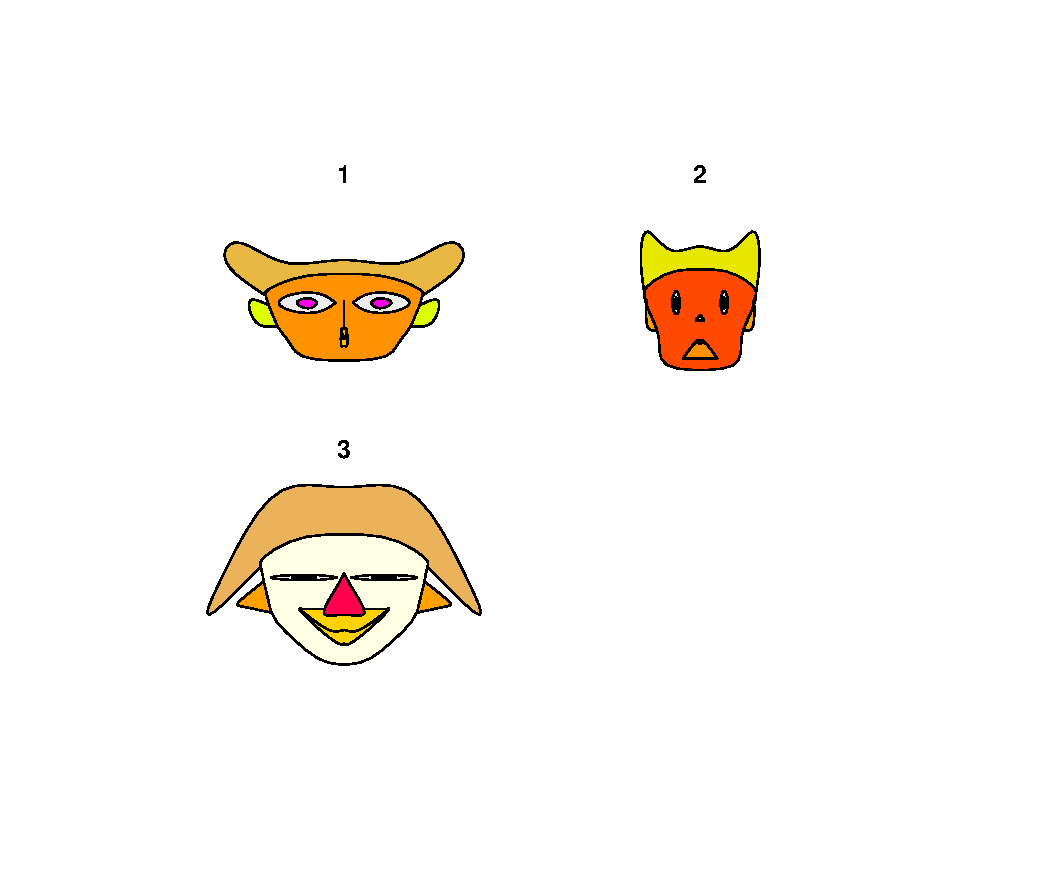
\includegraphics[width = \textwidth]{faces.eps}
		\caption{cheroff faces}
		\end{subfigure}
		\caption{display of different means of measurement for 3 time periods}
		\label{display_means}
	\end{figure}
\newpage
	\item 
	We use Hotelling's $T^2$ test to test the difference of mean vectors between period 1 and period 3.
	\begin{rcode}
## test for difference in skull sizes between period 1 and period 3
library(ICSNP)
T2test <- HotellingsT2(skulls[skulls$period == 1, -ncol(skulls)], skulls[skulls$period == 3, -ncol(skulls)], test = 'f')
	\end{rcode}
	The result is
	\begin{rcode}
#	Hotelling's two sample T2-test

data:  skulls[skulls$period == 1, -ncol(skulls)] and skulls[skulls$period == 3, -ncol(skulls)]
T.2 = 3.1744, df1 = 4, df2 = 55, p-value = 0.02035
alternative hypothesis: true location difference is not equal to c(0,0,0,0)
	\end{rcode}
Then we calculate the $T^2$ value
\begin{rcode}
df1 <- T2test$parameter['df1']
df2 <- T2test$parameter['df2']
T2stat <- T2test$statistic/df2*(df1 + df2 - 1)*df1
T2stat
\end{rcode}

So the $T^2$ statistic is \textbf{13.39036} and the p-value is \textbf{0.02035}. Thus with small p-value we reject the null hypothesis and conclude that there is significant evidence that the means of measurements are different between period 1 and period 3. 

Here our assumptions are:
\begin{itemize}[label = -]
 \item 
 multivariate normality for both period 1 and period 3;
 \item
 homogeneous variance covariance matrix for period 1 and period 3.
\end{itemize}

  For multivariate normality, we can justify this from the $\chi^2$ Q-Q plots in Figure~\ref{QQ} from part 1 and the formal test for multivariate normality in part 2(a). For homogeneous variance covariance matrix, we do a Box M test for period 1 and period 3, and the result shows that there is no significant evidence that they have different variance covariance matrix, thus the second assumption about homogeneous variance covariance matrix is also justified.
Box M test on homogeneity of variance covariance matrix for period 1 and period 3:
\begin{rcode}
BoxMTest(X = skulls[which(skulls$period == c(1,3)), -ncol(skulls)], cl = skulls$period[which(skulls$period == c(1,3))])  
\end{rcode}
The result:
\begin{rcode}
[1] 2

------------------------------------------------------------
 MBox F df1 df2 P
------------------------------------------------------------
   13.8566     1.1692         10          3748       0.3066
------------------------------------------------------------
Covariance matrices are not significantly different.
$MBox
       1 
13.85656 

$F
       1 
1.169162 

$df1
[1] 10

$df2
[1] 3748

$pValue
        1 
0.3066301 
\end{rcode}
The p-value is big and we fail to reject the null hypothesis and conclude that there is no significant difference in the variance covariance matrix for period 1 and period 3.

\item 
One-way MANOVA using 3 time periods (here SAS contrast is adopted):
\begin{rcode}
## one-way MANOVA of skulls
library(car)
fit.lm <- lm(cbind(`max breadth`, `basibregmatic height`, `basialveolar length`, `nasal height`) ~ period, data = skulls, contrasts = list(period = contr.SAS))
fit.manova <- Manova(fit.lm)

summary(fit.manova)
\end{rcode}
The result is:
\begin{rcode*}{fontsize = \footnotesize}
Type II MANOVA Tests:

Sum of squares and products for error:
                     max breadth basibregmatic height basialveolar length nasal height
max breadth            1785.4000                172.5            128.9667     289.6333
basibregmatic height    172.5000               1924.3            178.8000     171.9000
basialveolar length     128.9667                178.8           2153.0000      -1.7000
nasal height            289.6333                171.9             -1.7000     840.2000

------------------------------------------
 
Term: period 

Sum of squares and products for the hypothesis:
                     max breadth basibregmatic height basialveolar length nasal height
max breadth           150.200000            20.300000          -161.83333     5.033333
basibregmatic height   20.300000            20.600000           -38.73333     6.433333
basialveolar length  -161.833333           -38.733333           190.28889   -10.855556
nasal height            5.033333             6.433333           -10.85556     2.022222

Multivariate Tests: period
                 Df test stat approx F num Df den Df    Pr(>F)   
Pillai            2 0.1722118 2.002148      8    170 0.0489045 * 
Wilks             2 0.8301027 2.049069      8    168 0.0435825 * 
Hotelling-Lawley  2 0.2018820 2.094526      8    166 0.0389623 * 
Roy               2 0.1869691 3.973094      4     85 0.0052784 **
---
Signif. codes:  0 ‘***’ 0.001 ‘**’ 0.01 ‘*’ 0.05 ‘.’ 0.1 ‘ ’ 1
\end{rcode*}

With small p-value, we conclude that the mean vectors of 4 measurements are different for the 3 time periods. The assumptions are also multivariate normality and homogeneous variance covariance matrix for the 3 periods, which can be justified by answers in part 1 and part 2.


\item 
\begin{enumerate}
	\item Now we test if there are any changes in the mean vectors from period 1 to period 2 and period 2 to period 3 respectively. Since we use the SAS contrast, in mean vectors for 3 time periods, $\bm \mu_{k} = \bm \mu + \bm \tau_k,\, k = 1, 2, 3$, we have $\bm \tau_3 = \bm 0$. Thus
	\[
		\bm \mu_1 - \bm \mu_2 = \bm \tau_{1} - \bm \tau_{2} = \begin{bmatrix}
		 0 & 1 & -1
	\end{bmatrix} \begin{bmatrix}
		\bm \mu\\
		\bm \tau_{1}\\
		\bm \tau_{2}
	\end{bmatrix}\]
	and
	\[
		\bm \mu_{2} - \bm \mu_3 = \bm \tau_{2} = \begin{bmatrix}
		 0 & 0 & 1
	\end{bmatrix} \begin{bmatrix}
		\bm \mu\\
		\bm \tau_{1}\\
		\bm \tau_{2}
	\end{bmatrix}\]
	Hence our tests are using $C_{12} = \begin{bmatrix}
		0 & 1 & -1
	\end{bmatrix}$ and $C_{23} = \begin{bmatrix}
		0 & 0 & 1
	\end{bmatrix}$ as our hypothesis matrix.

	\begin{rcode}
## test mean vector changes from period 1 to period 2
C12 <- matrix(c(0,1,-1),nrow = 1, byrow = T)
test12 <- linearHypothesis(model = fit.lm, hypothesis.matrix = C12)

## test mean vector changes from period 2 to period 3
C23 <- matrix(c(0,0,1),nrow = 1, byrow = T)
test23 <- linearHypothesis(model = fit.lm, hypothesis.matrix = C23)
\end{rcode}
The results are:

for period 1 to period 2:
\begin{rcode*}{fontsize = \footnotesize, breaklines = false}
Sum of squares and products for the hypothesis:
                     max breadth basibregmatic height basialveolar length nasal height
max breadth                 15.0               -13.50               -1.50        -4.50
basibregmatic height       -13.5                12.15                1.35         4.05
basialveolar length         -1.5                 1.35                0.15         0.45
nasal height                -4.5                 4.05                0.45         1.35

Sum of squares and products for error:
                     max breadth basibregmatic height basialveolar length nasal height
max breadth            1785.4000                172.5            128.9667     289.6333
basibregmatic height    172.5000               1924.3            178.8000     171.9000
basialveolar length     128.9667                178.8           2153.0000      -1.7000
nasal height            289.6333                171.9             -1.7000     840.2000

Multivariate Tests: 
                 Df test stat  approx F num Df den Df  Pr(>F)
Pillai            1 0.0187978 0.4023169      4     84 0.80648
Wilks             1 0.9812022 0.4023169      4     84 0.80648
Hotelling-Lawley  1 0.0191579 0.4023169      4     84 0.80648
Roy               1 0.0191579 0.4023169      4     84 0.80648
\end{rcode*}

for period 2 to period 3:
\begin{rcode*}{fontsize = \footnotesize, breaklines = false}
Sum of squares and products for the hypothesis:
                     max breadth basibregmatic height basialveolar length nasal height
max breadth                66.15                34.65           -95.55000    10.500000
basibregmatic height       34.65                18.15           -50.05000     5.500000
basialveolar length       -95.55               -50.05           138.01667   -15.166667
nasal height               10.50                 5.50           -15.16667     1.666667

Sum of squares and products for error:
                     max breadth basibregmatic height basialveolar length nasal height
max breadth            1785.4000                172.5            128.9667     289.6333
basibregmatic height    172.5000               1924.3            178.8000     171.9000
basialveolar length     128.9667                178.8           2153.0000      -1.7000
nasal height            289.6333                171.9             -1.7000     840.2000

Multivariate Tests: 
                 Df test stat approx F num Df den Df   Pr(>F)  
Pillai            1 0.1061197 2.493079      4     84 0.049056 *
Wilks             1 0.8938803 2.493079      4     84 0.049056 *
Hotelling-Lawley  1 0.1187181 2.493079      4     84 0.049056 *
Roy               1 0.1187181 2.493079      4     84 0.049056 *
---
Signif. codes:  0 ‘***’ 0.001 ‘**’ 0.01 ‘*’ 0.05 ‘.’ 0.1 ‘ ’ 1
\end{rcode*}
From the results, we can see from period 1 to period 2, there is no significant evidence that any changes happened since the p-value is big. However, from period 2 to period 3, we have evidence that there are some changes with p-value less than 0.05. 

\item 
we test simultaneously at the 99\% level of significance the difference of 4 means of measurements from period 1 to period 2 and from period 2 to period 3 (8 tests). Then we adjust the p-values with Bonferroni.
\begin{rcode}
## simutanous tests: 4 measurements and 1-2, 2-3 periods. (8 pairs)
n <- table(skulls$period)
S_pool <- fit.manova$SSPE/fit.manova$error.df
mean_diff_12 <- fit.lm$coefficients[2,] - fit.lm$coefficients[3,]
mean_diff_23 <- fit.lm$coefficients[3,]
S_pool_ii <- diag(S_pool)
t_12 <- abs(mean_diff_12)/sqrt(((1/n[1]) + (1/n[2]))*S_pool_ii)
t_23 <- abs(mean_diff_23)/sqrt(((1/n[2]) + (1/n[3]))*S_pool_ii)
Tstat <- rbind(t_12, t_23)
row.names(Tstat) <- c("12", "23")

p_vals <- 2*pt(Tstat, df = fit.manova$error.df, lower.tail = F)
p.adjust(p_vals, "bonferroni")
\end{rcode}
The adjusted p-values are:
\begin{rcode}
1.0000000 0.6085210 1.0000000 1.0000000 1.0000000 0.1634379 1.0000000 1.0000000
\end{rcode}
So none of the simutaneous tests is significant at 1\% level of significance. None of the mean component changes from period 1 to period 2 or period 2 to period 3 in this test.

\item 
We construct 8 simutaneous 95\% confidence inertvals. 
\begin{rcode}
## simutanous tests confidence interval: period 1 to period 2 ((4 out of 8 simutaneous pairs))
alpha1 <- 0.05
m <- 8

margin12 <- qt(1 - alpha1/(2*m), df = fit.manova$error.df)*sqrt(((1/n[1]) + (1/n[2]))*S_pool_ii)
conf.int12 <- rbind(mean_diff_12 - margin12, mean_diff_12 + margin12)

## simutanous tests confidence interval: period 2 to period 3 (4 out of 8 simutaneous pairs)
margin23 <- qt(1 - alpha1/(2*m), df = fit.manova$error.df)*sqrt(((1/n[2]) + (1/n[3]))*S_pool_ii)
conf.int23 <- rbind(mean_diff_23 - margin23, mean_diff_23 + margin23)
  \end{rcode}  
  Then the 8 intervals are (the first row is lower bound of the interval and the second row is the upper bound of the interval):
 \begin{rcode*}{fontsize = \footnotesize}
     max breadth basibregmatic height basialveolar length nasal height
[1,]    -4.27801            -2.503133           -3.499685    -1.948712
[2,]     2.27801             4.303133            3.699685     2.548712
     max breadth basibregmatic height basialveolar length nasal height
[1,]    -5.37801            -4.503133           -0.566352    -2.582045
[2,]     1.17801             2.303133            6.633019     1.915379
 \end{rcode*}
 We can see all the simutaneous intervals contain 0. Hence we do not have significant evidence that there is any change for any of the 4 measurements over the two time periods.


\end{enumerate}


 	\end{enumerate}









	
	
	
	\end{document}